%about the sensor node...

The sensor node provides data about the current state of the flower environment to the controller.
It has been developed as a low power device which guarantees long battery duration.
Arduino has been chosen as platform for this node because of its powerful libraries and support. Also the microcontroller has to offer sufficient ADCs and GPIO pins to access all required modules such as communication chip, real time clock and sensors. Other platforms such as XBee could not be used, as they do not directly support protocols such as TWI. Also they are expensive.
In particular we chose the Arduino Mini 3.3V 8MHz board, as it is the most basic board and therefore offering the lowest power consumption. Further details about minimizing the power consumption are explained in \ref{sec:lowpower}.



The sensors used are:
\begin{itemize}

\item \textbf{DHT11 - Temperature and humidity sensor}\\
The datasheet claims this sensor reaches a repeatability of $\pm0.2°C$ for the temperature and an accuracy of $\pm 5\%$ for humidity. It seems to be a widely used sensor for arduino projects, however in operation its humidity accuracy was far worse than promised by the manufacturer and a cumbersome calibration of the sensor is needed. Further research showed that it is not always a reliable humidity sensor and probably should be replaced by the more expensive DHT22 or other alternatives. We kept the sensor in the setup, however no decision has been based on its data.

\item \textbf{Moisture sensor}\\
We tried two types of moisture sensors. A resistance based sensor and a capacitive sensor. The electrodes used for the resistance sensors interact with the water in the soil as current flows. This pollutes the soil and destroys the sensor over time. Performing only sporadic measurements postpones this effect, however it cannot be avoided. Capacitive sensors do not interact with the soil as they measure the humidity through the capacity of the soil, not its resistance. So no current flows through the soil and there are no metallic or corrosive electrodes.\\

The resistance based sensor consists of two parts, the resistance probe (YL-69) and a control board (YL-38). The probe will be put into the measured soil, while the board should stay dry. It provides an analog signal. The ATmega328 has a 10 bit ADC, so the result read from the ADC is an integer between 0 and 1023.\\

The test showed that in a dry state the sensor shows 1023. Connecting the electrodes with a finger leads to a value around 1000.\\
Also in dry soil the readout is 1023, but as we pour water into the pot, it continuously decreases down to a few hundred.\\

We might have to calibrate the moisture levels for different flower or soil types, but in general the sensor seems to do the job very well.\\

The capacitive sensor used is the SEN0193. It is handled the same way as the YL-69 sensor on the software side, however it does not influence the soil.




\item \textbf{Brightness sensor}\\
To gather information about the brightness in the environment, a photoresistor has been used. This is a semiconductor that reacts to light. The manual of the sensor suggested the range of the photoresistor is between 500$\Omega$ (bright) and 50$k\Omega$ (dark). 
Further it suggested to use a 1$k\Omega$ resistor for the voltage divider. An arduino tutorial \citep{misc:photoresistor_tutorial} suggested 10 $k\Omega$. So we decided to measure the actual resistor values and use the formula from the lecture to calculate the matching resistor of the voltage divider. % , 26$k\Omega$ was a good choice  

The measurements showed that the actual photoresistor range is 500$\Omega$ to 1.7$M\Omega$.\\
\begin{equation}
R_1 = \sqrt{R_{max}*R_{max}} = \sqrt{500*1700000} = \sqrt{850000000} = 29k\Omega
\end{equation}


The closest resistor available to us was 26$k\Omega$.\\
These values differ to those suggested by the tutorials, but since also the photoresistor has different values, our choice seems feasible. Also we are convinced a higher resistor will not harm the components and result in lower power consumption in contrast to a small resistor.\\
So we connected the chosen pulldown resistor between ground and an ADC pin of the Arduino. To complete the voltage divider the photoresistor was connected between VCC and the ADC pin.\\

The sensor worked very well in the tests and showed a value between 30 (covered sensor) and 950 (next to a light bulb). That confirmed our choice of the resistor.\\


\item \textbf{Battery Voltage Sensor}\\
As the sensor node is powered by a battery it is good to have information about the battery status.
This can be done by measuring the voltage of the battery via a voltage divider. There are two ways of setting the voltage reference of the ADC unit. Either the VCC of the ATmega or the internal reference voltage of 1.1V can be used.
The former has the advantage of higher accuracy, assuming a stable supply voltage. However a supply voltage lower than 3.3V cannot be measured correctly. Notice that the ATmega328 will continue to operate even at a supply voltage as low as 2.7V, although some external components might fail.
 The second version has the advantage that also supply voltages below 3.3V can be measured, however it has to be calibrated for each ATmega individually to be as precise.

In any case a voltage divider is needed to convert the voltage from 0-6V to 0-3.3V respectively 0-1.1V. The design of the voltage divider is a trade\-off between measurement precision and power consumption. \cite{misc:battery_voltage_measurement} If its total resistance is low, the power consumption of the voltage divider is too high for a low power device. If the resistance is too high, the measurement will become unstable and a capacitor becomes necessary to smooth the measurements. We decided to use a resistance of $100k\Omega$ between GND and the ADC pin as well as $500k\Omega$ between VCC and the ADC pin. This seemed to be a good trade-off without requiring a capacitor.

% Ezio: 
% VCC - 1MO - ADC - 39kO - (1MO / 470kO) - 22kO - GND (1MO / 381kO)

% Ours:
% VCC - 500kO - ADC - 108kO - GND 			(500kO / 100kO)





\end{itemize}


\subsubsection{Low Power Capability}
\label{sec:lowpower}

As mentioned before, the Arduino Mini 3.3V 8MHz is the basis of our sensor node platform. However the Arduino uses about 6 mA in standby. With this current consumption a set of batteries (assuming a capacity of 2000mAh) would be empty within 14 days. In a network consisting of 7 sensor nodes, every second day batteries would be needed to be changed. This motivates to look into further power saving techniques for the Arduino.\\

\subsubsection{Power supply}

One of the obvious questions is the supply of the operating voltage. It has been looked into the following options:

\begin{itemize}
\item \textbf{Using the Arduino voltage regulator}
The Arduino board can be powered directly from the battery and generate its own supply voltage.
However this regulator is very inefficient.

\item \textbf{Using an external voltage regulator}
A more efficient external regulator can be used instead of the onboard regulator. The original regulator will still consume a small current, even if not used. Therefore it should be removed in this case. The external regulator will require a supply voltage of typically 100-200mV above the output voltage. The regulator tested by us, MCP1700-3302E, needs 3.5V, so in case of three batteries this is 1.17V per battery.\\
During the discharge process of a battery its output voltage drops. Once the voltage drops under the required supply voltage of a voltage regulator, the output voltage of the regulator will not match 3.3V anymore.\\
Figure \ref{fig:dischage_curve} illustrates the battery voltage of a AA NiMH battery over different loads. %It is important to notice that with a low load the battery voltage stays above 1.17V for a longer period.
It is important to notice that with a low load the ampere hours obtained from the battery increases. So decreasing the current used by the system by half results in more than just doubled battery life.
In our application the load is less than 1mA with some 15mA pulses during data transmission. This is even far less than the uppermost line indicates. It can be concluded that the energy remaining in the battery once its voltage drops below 1.17V is less than 400mA.

\item \textbf{Using a buck-boost converter}
A conventional voltage regulator needs a supply voltage of at least little over 3.3V to provide a 3.3V output.
A buck-boost converter like the Pololu reg 12a which we tested, can convert voltages above 0.5V to constant 3.3V.\\
This is beneficial because of the dropping battery voltage during the discharge process. 
A buck-boost converter has a lower required supply voltage (0.5V) and therefore gets nearly all energy out of the battery. However it turned out that for very low currents, like in our sensor node, the power consumed by the Pololu is much higher than for the linear voltage regulator. This diminishes the advantage of the Pololu and even turns it into the worse choice in terms of energy efficiency. Regarding costs the linear power regulator beats the pololu by an order of magnitude.

\end{itemize}


\begin{figure}[htbp]
\begin{center}
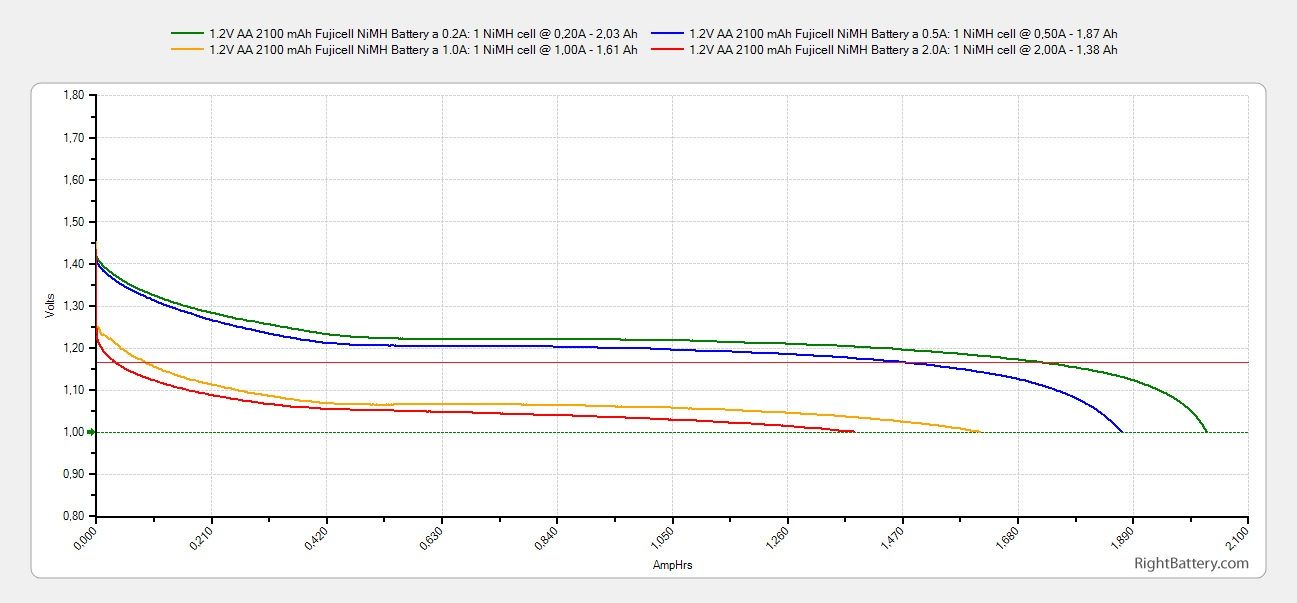
\includegraphics[width=1.0\columnwidth]{images/discharge_curves.jpg}
\end{center}
\caption{Discharge curves over different currents}
\label{fig:dischage_curve}
\end{figure}


We tried all solutions in our tests, however for the final solution we recommend the linear voltage regulator with adequate batteries (3 x 1.5V or 4 x 1.2V).

\subsubsection{Power consumption optimizations}
To make the batteries last as long as possible, the node should use as little power as possible.\\
The biggest power safer is to put the microcontroller and all peripheral devices including all sensors into sleep mode as much as possible.\\
This reduces the power of the system to around 1.5mA and gives 8 weeks of battery life per node. This is a big improvement, however far away from a convenient solution and the technical limits.\\
One further optimization is to remove the power LED used to indicate the Arduino is running, as there is no need for it and the LED uses a lot of power. The LED can be removed by adding tin to connect both legs, heating them up uniformly and pulling away the LED with tweezers. This decreases the consumption to about 0.26 mA (45 weeks). \\
Disabling TWI before sleep saved another 170µA.\\
Removing the parasiting onboard voltage regulator saved further 75µA. However de-soldering of medium sized SMD components requires special equipment, skills or patience.\\
The resulting consumption for the design including all final components and using the external voltage regulator is 15µA. (4.5V ==> 67.5µW)
Using the Pololu the same design needs 90µA (4.5V ==> 405µW).
It can be concluded that in this situation an appropriate voltage regulator is more efficient than a Pololu. Also the voltage divider is a far cheaper solution.\\

\paragraph{Battery}
One crucial factor obviously is the kind of battery itself. The following summarizes the key issues of batteries in our application.
\begin{itemize}
\item \textbf{Voltage}\\
It must be mentioned that every battery type operates at a different voltage, what has to be considered at the choice of battery.
Three 1.5V alkaline batteries have been assumed in the calculations above, resulting in 4.5V total. Using rechargeable batteries with 1.2V each, like nickel metal hydride batteries, the resulting total 3.6V are just slightly above the threshold for the voltage regulator to operate, so they will fail very soon. In this case the Pololu would have the better performance. For operation with the voltage regulator 3x1.5V LSD NiMH batteries or 4x1.2V rechargeable alkaline batteries are recommended.

\item \textbf{Capacity}\\
Obviously batteries with higher capacity last longer without replacing them.

\item \textbf{Temperature range}\\
Not all batteries withstand extreme temperatures. For example conventional NiMH batteries are not supposed to be used in cold environments, while their self-discharge rate drastically increases at high temperatures. LSD NiMH however can resist cold temperatures.

\item \textbf{Self discharge rate}\\
Conventional NiMH batteries have a high self discharge rate. Even if not used, they loose half their energy after one month. Low self discharge NiMH (LSD NiMH) batteries loose only a fraction of this energy per month $(<3\%)$ and can be used for several years without recharging.
\end{itemize}


\subsubsection{PCB}
In order to incorporate all components into a small box, a PCB has been designed by our supervisor using the Fritzing tool. The yellow traces are on the top side and the orange traces on the bottom. To offer flexibility with the power supply of the sensors, it can be selected whether they should be powered by the normal VCC pin or powered by an arduino pin to be able to deactivate all sensors during low power phases.
The board has been produced by the Fritzing company tested with our software. It works as expected.
\begin{figure}[h!]
	\begin{center}
%	\includegraphics[scale=2]{images/PlantSensorPCB.pdf}
	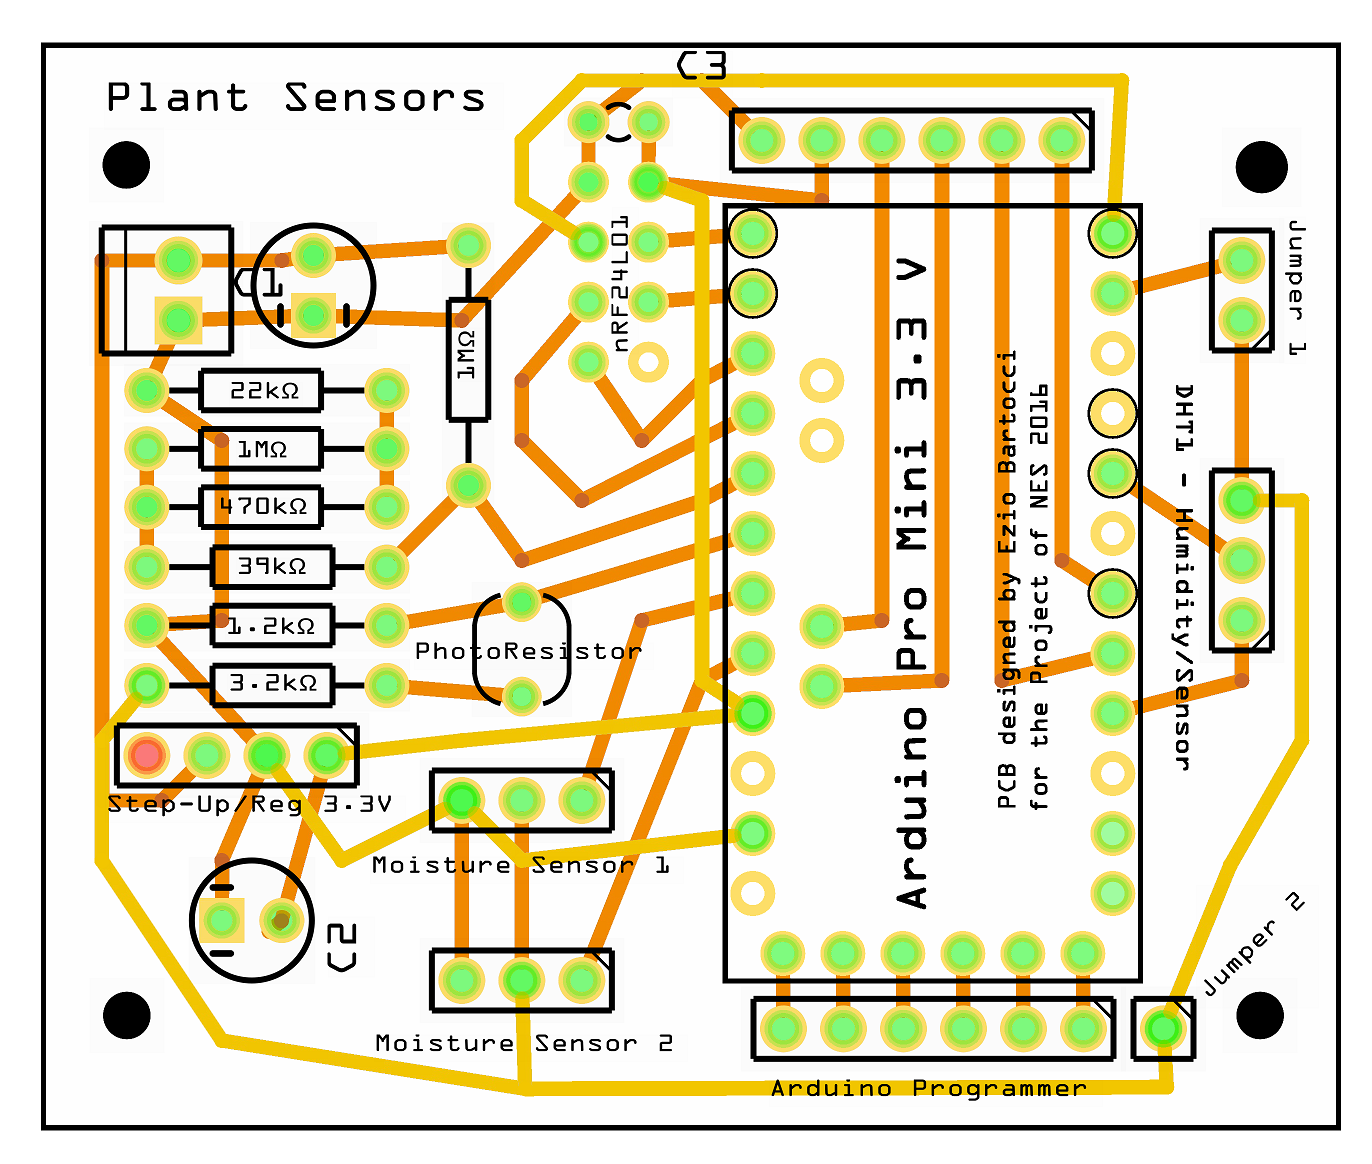
\includegraphics[scale=0.3]{images/SensorNode_small.png}
	
	\caption{PCB design of the sensor node.}
	\label{Setup_overview}
	\end{center}
\end{figure}

\subsubsection{Data storage}
As the communication between a sensor node and the controller might be faulty, the data shouldn't get lost. If the sensor node sends data to the controller and doesn't get a response, the data is stored in the EEPROM of the sensor node until the controller requests the data.
The size of the EEPROM is limited to 1KB, therefore only around 25 data sets fit into the storage.
Another issue with using EEPROM as storage is that the write cycles it endures are limited. Therefore an algorithm has been developed to ensure equal wearout of the EEPROM cells. In case the controller does not request the data and the EEPROM memory is full, the oldest data in the storage is replaced with the most recent data. 

\subsubsection{State diagram}

\begin{figure}[H]
	\begin{center}
	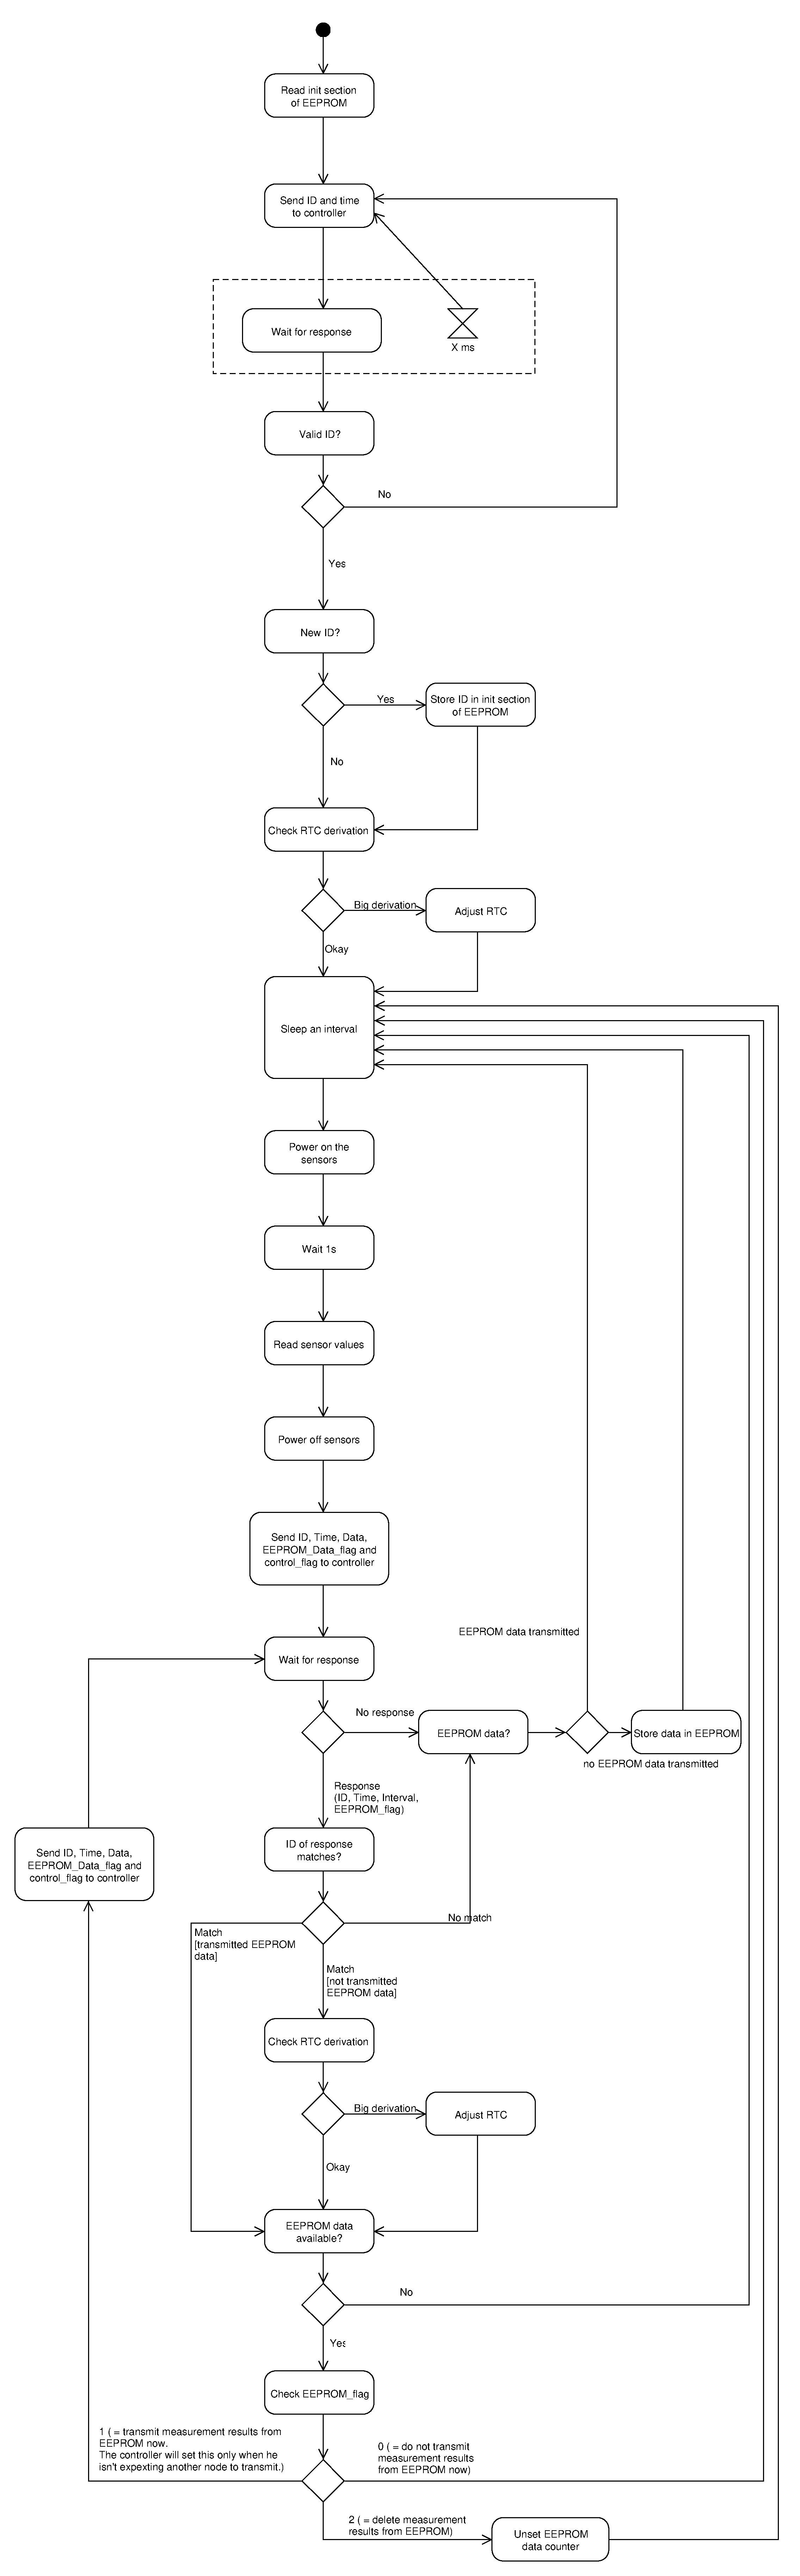
\includegraphics[scale=0.18]{images/SensorNode_0_4.pdf}
	\caption{State diagram of the sensor node.}
	\label{Setup_overview}
	\end{center}
\end{figure}